\documentclass[10pt,a4paper]{report}
\usepackage[utf8]{inputenc}
\usepackage[T1]{fontenc}
\usepackage{amsmath}
\usepackage{amsfonts}
\usepackage{amssymb}
\usepackage{makeidx}
\usepackage{graphicx}
\usepackage{url}
\usepackage[top=0.5cm]{geometry}
\begin{document}
\begin{figure}[t]
\includegraphics[width=15cm, height=5cm]{Prob}
Prawdopodobieństwo na matematyce dyskretnej
\end{figure}
Warto\'sć oczekiwana\\
Niech X będzie zmienną losową typu dyskretnego. Wartością oczekiwaną nazywa się sumę iloczynów wartości tej zmiennej losowej oraz prawdopodobieństw z jakimi są one przyjmowane.\\
Jeżeli dyskretna zmienna losowa X przyjmuje wartości $x_1, x_2, \dots, x_n$ z prawdopodobieństwami wynoszącymi odpowiednio $p_1, p_2, \dots, p_n$, to wartość oczekiwana $\mathbb EX$ zmiennej losowej X wyraża się wzorem
\begin{equation}\label{EX}
\mathbb EX = \sum_{i=1}^n x_i p_i.
\end{equation}
Wariancja – klasyczna miara zmienności.\\
 Intuicyjnie utożsamiana ze zróżnicowaniem zbiorowości; jest średnią arytmetyczną kwadratów odchyleń (różnic) poszczególnych wartości cechy od wartości oczekiwanej.\\
Wariancja zmiennej losowej  X , oznaczana jako  $\operatorname{Var}[X]$  lub  $D^2 (X)$ , zdefiniowana jest wzorem:
\begin{equation*}
\operatorname{Var}[X]=\mathbb E[(X-\mu)^2],
\end{equation*}
gdzie:\\
$\mathbb E[\dots ]$ to warto\'sć oczekiwana~(\ref{EX}) zmiennej losowej podanej w nawiasach kwadratowych,\\
$\mu$; jest wartością oczekiwaną zmiennej X.\cite{Wariancja}\\
\underline{Przykład}\\
Obliczymy wariancje dla rzutu symetryczną kostką do gry\\
\begin{eqnarray*}
D^2(X)=\mathbb E[(X-\mathbb EX)^2]=\mathbb E(X^2)- (\mathbb EX)^2=\\
=\sum_{i=1}^{6}\frac{i^2}{6}-(\sum_{i=1}^{6}\frac{i}{6})^2=\frac{1+4+9+16+25+36}{6}\\
-(\frac{1+2+3+4+5+6}{6})^2=\frac{91}{6}-\frac{49}{4}=\frac{35}{12}
\end{eqnarray*}
Dystrybuanta\\
Niech $\mathbb{P}$ będzie rozkładem prawdopodobieństwa na prostej. Funkcję $F\colon\mathbb R \to \mathbb R$ daną wzorem
\begin{equation}\label{F}
F(t)=\mathbb{P}((-\infty ,t])
\end{equation}
nazywamy dystrybuantą rozkładu $\mathbb P$.\cite{Dystrybuanta}
\begin{figure}[b]
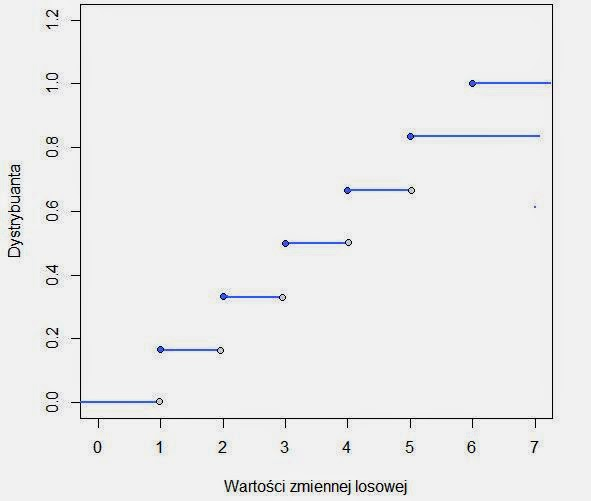
\includegraphics[width=7cm, height=3cm]{Dystrybuanta}
Dystrybuanta (\ref{F}) dla rzutu kostką 
\end{figure}
\begin{array}{|l|cr}
left1 & center1 & right1\\
\hline
d & e & f
\end{array}
\begin{thebibliography}{2}
\bibitem{Wariancja}
\url{https://pl.wikipedia.org/wiki/Wariancja}
\bibitem{Dystrybuanta}
\url{https://pl.wikipedia.org/wiki/Dystrybuanta}
\end{thebibliography}
\end{document}